% Apresentação final da PoC OCR-06 no Workshop LabREC (INE5448), 15 min + 5 min de perguntas
\documentclass[aspectratio=169,11pt]{beamer}
\usetheme{metropolis}
\usepackage[utf8]{inputenc}
\usepackage[T1]{fontenc}
\usepackage[brazil]{babel}
\usepackage{booktabs}
\usepackage{xcolor}
\usepackage{array}
\usepackage{tikz}
\usetikzlibrary{positioning,arrows.meta}
\metroset{progressbar=frametitle, numbering=fraction}
\setbeamertemplate{caption}{\insertcaption}
\graphicspath{{../apresentacao_final/figs/}{../POC/figs/}{figs/}}
\definecolor{bom}{HTML}{1B8A62}
\definecolor{ruim}{HTML}{C0392B}
\definecolor{tinta}{HTML}{52514E}
\newcommand{\ok}[1]{\textcolor{bom}{#1}}
\newcommand{\erro}[1]{\textcolor{ruim}{#1}}

\title{OCR-06: OCR Adaptativo com Aprendizagem Assistida}
\subtitle{Leitura de nomes manuscritos em certidões de Registro Civil}
\author{Gabriel Salmoria \quad {\small Tutor: Lucas Mayr}}
\institute{INE5448 -- IA e Segurança -- UFSC \quad Workshop LabREC}
\date{Novembro de 2026}

\begin{document}

\maketitle

% ================================================================== abertura
\begin{frame}{Nomes raros são o ponto fraco do OCR}
\begin{columns}[T]
\begin{column}{0.52\textwidth}
\small
\textbf{Problema}
\begin{itemize}
  \item OCRs baseados em modelos de linguagem leem bem o texto comum, mas trocam um nome raro pelo mais provável
  \item Num registro, uma letra errada no nome já é um erro no documento
\end{itemize}
\vspace{0.4em}
\textbf{Objetivo}
\begin{itemize}
  \item Ajustar um OCR aberto para ler melhor os campos manuscritos, principalmente nomes que ele nunca viu
  \item Sem treinar com dados de pessoas reais
\end{itemize}
\end{column}
\begin{column}{0.45\textwidth}
\centering
\vspace{0.6em}
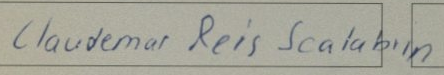
\includegraphics[width=0.85\linewidth]{nome_1.png}

\vspace{0.6em}
\footnotesize
\begin{tabular}{@{}ll@{}}
Escrito & Claudemar Reis Scalabrin \\
Chandra & Claude\erro{mi}r Reis Scalabrin \\
Ajustado & \ok{Claudemar Reis Scalabrin} \\
\end{tabular}
\end{column}
\end{columns}
\end{frame}

\begin{frame}{Trajetória do projeto}
\centering
\begin{tikzpicture}[
    font=\small,
    etapa/.style={draw=tinta, rounded corners=3pt, align=center, text width=2.75cm, minimum height=1.9cm, fill=white},
    data/.style={font=\scriptsize\bfseries, text=tinta},
    res/.style={font=\scriptsize, align=center, text width=2.75cm},
    arr/.style={-{Stealth[length=2.2mm]}, thick, draw=tinta}]
  \node[etapa] (p) {\textbf{Proposta}\\ajuste LoRA de um OCR aberto};
  \node[etapa, right=0.55cm of p] (d) {\textbf{Dados}\\nomes públicos e linhas sintéticas};
  \node[etapa, right=0.55cm of d] (l) {\textbf{Etapa 1: linhas}\\adaptador lora\_v0};
  \node[etapa, right=0.55cm of l, fill=bom!12] (g) {\textbf{Etapa 2: páginas}\\lora\_v1, lora\_v2, FP8 e INT4};
  \foreach \a/\b in {p/d, d/l, l/g} \draw[arr] (\a) -- (\b);
  \node[data, above=0.15cm of p] {set.};
  \node[data, above=0.15cm of d] {out.};
  \node[data, above=0.15cm of l] {nov.};
  \node[data, above=0.15cm of g] {nov.};
  \node[res, below=0.25cm of p] {nomes raros, sem dados pessoais};
  \node[res, below=0.25cm of d] {46 mil linhas sintéticas e 26 mil reais (BRESSAY)};
  \node[res, below=0.25cm of l] {CER no BRESSAY: 20,1\% $\rightarrow$ 4,9\%};
  \node[res, below=0.25cm of g] {campos manuscritos certos: 55\% $\rightarrow$ 72\%};
\end{tikzpicture}

\vspace{1.2em}
\raggedright
\small
O modelo base é o \textbf{Chandra OCR 2}, OCR aberto derivado do Qwen3.5-4B, que transcreve a página inteira em HTML com a posição de cada bloco. Todos os ajustes são LoRA (0,7\% dos parâmetros).
\end{frame}

% ================================================================== etapa 1: linhas
\begin{frame}{Etapa 1: nomes reais, mas só como contagens por palavra}
\begin{columns}[T]
\begin{column}{0.47\textwidth}
\small
\begin{itemize}
  \item \textbf{Léxico}: 100 mil prenomes (IBGE), 61 mil sobrenomes (TSE e Receita) e 5.570 municípios, só como contagens por palavra
  \item \textbf{Linhas sintéticas}: nomes sorteados pela frequência real, em 85 fontes manuscritas, com degradação de papel escaneado
  \item \textbf{BRESSAY}: redações manuscritas reais, separadas por autor entre treino e teste
\end{itemize}
\end{column}
\begin{column}{0.51\textwidth}
\centering
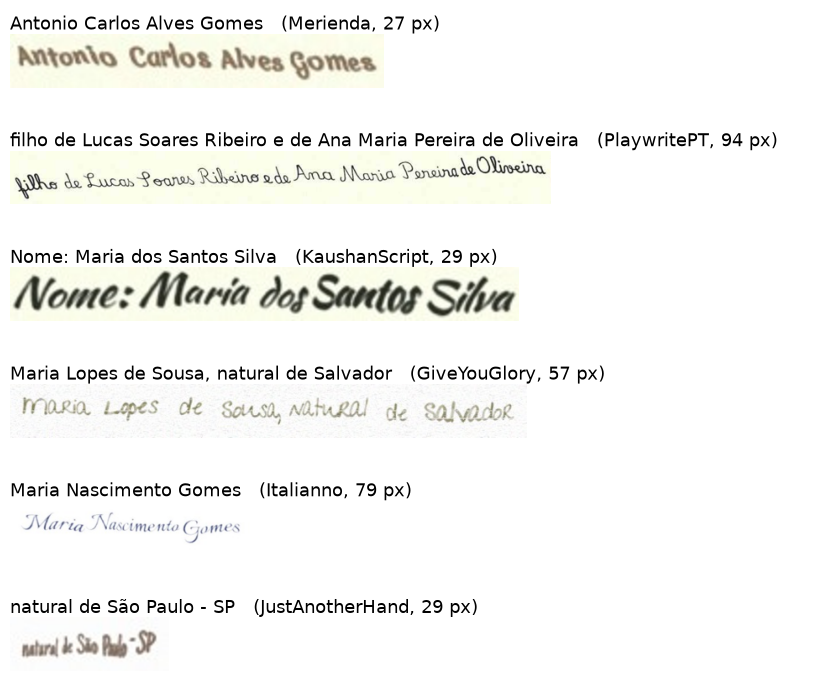
\includegraphics[height=0.66\textheight]{exemplos_linhas.png}

\scriptsize Linhas sintéticas, com o rótulo e a fonte acima de cada uma
\end{column}
\end{columns}
\end{frame}

\begin{frame}{Em linhas, o erro no manuscrito real caiu para um quarto}
\centering
\small
\begin{tabular}{@{}lrr@{}}
\toprule
& Chandra OCR 2 & Ajustado (lora\_v0) \\
\midrule
\multicolumn{3}{@{}l}{\textit{BRESSAY: 5.146 linhas de autores fora do treino}} \\
\quad CER (\%) $\downarrow$ & 20,1 & \textbf{4,9} \\
\quad Linhas sem nenhum erro (\%) & 12,6 & \textbf{33,5} \\
\multicolumn{3}{@{}l}{\textit{Sintético: 4.000 linhas, fontes e nomes fora do treino}} \\
\quad CER (\%) $\downarrow$ & 8,6 & \textbf{3,4} \\
\quad Nomes nunca vistos lidos sem erro (\%) & 70,9 & \textbf{79,7} \\
\quad Diferença de CER entre nomes vistos e inéditos (pontos) & 2,3 & 2,1 \\
\bottomrule
\end{tabular}

\vspace{0.8em}
\raggedright
\begin{itemize}
  \item A diferença entre nomes vistos e inéditos não aumentou: sem sinal de que o modelo decorou os nomes do treino
  \item A versão FP8 ficou a 0,1 ponto de CER da BF16 e foi de 16\% a 21\% mais rápida
\end{itemize}
\end{frame}

\begin{frame}{Em páginas inteiras, o ajuste em linhas quase não apareceu}
\small
O mesmo adaptador de linhas, aplicado em certidões inteiras:
\vspace{0.4em}

\centering
\begin{tabular}{@{}lrr@{}}
\toprule
Campos manuscritos exatos, página inteira & Chandra & Ajustado em linhas \\
\midrule
Certidões do OCRSD (47 págs.) & 84,7\% & 84,4\% \\
Certidões geradas localmente (38 págs.) & 56,6\% & 55,4\% \\
\quad só nomes & 19,9\% & 22,7\% \\
\bottomrule
\end{tabular}

\vspace{0.6em}
\raggedright
\begin{itemize}
  \item O Chandra é usado com a página inteira, e o adaptador só tinha visto recortes de uma linha
  \item Decisão: treinar com \textbf{páginas inteiras}, no formato HTML que o Chandra já produz
\end{itemize}
\end{frame}

% ================================================================== etapa 2: páginas
\begin{frame}{Etapa 2: treinar com páginas inteiras de certidões}
\begin{itemize}
  \item \textbf{Dados}: 1.000 páginas do OCRSD, o gerador de certidões sintéticas do ONR, e 2.500 geradas localmente, em 5 documentos de Registro Civil: casamento (antiga e CNJ), nascimento (CNJ), óbito e DNV
  \item \textbf{Alvo}: o HTML de layout do Chandra, com o texto impresso tirado da própria saída dele
  \item \textbf{Perda ponderada}: texto impresso com peso 0,3, manuscrito 1 e, no lora\_v2, nomes com peso 2 e peso extra quando o modelo erra uma letra
  \item \textbf{Duas etapas}: lora\_v1 (1.800 páginas) e lora\_v2 (mais 1.700), cerca de 65 min cada numa RTX PRO 6000, das páginas mais limpas às mais degradadas
  \item \textbf{Teste}: 200 páginas fora do treino, 100 \emph{difíceis} (70\% das palavras de nome nunca vistas) e 100 \emph{normais} (nomes pela frequência real)
\end{itemize}
\end{frame}

\begin{frame}{Como as páginas locais são geradas}
\begin{columns}[T]
\begin{column}{0.33\textwidth}
\centering
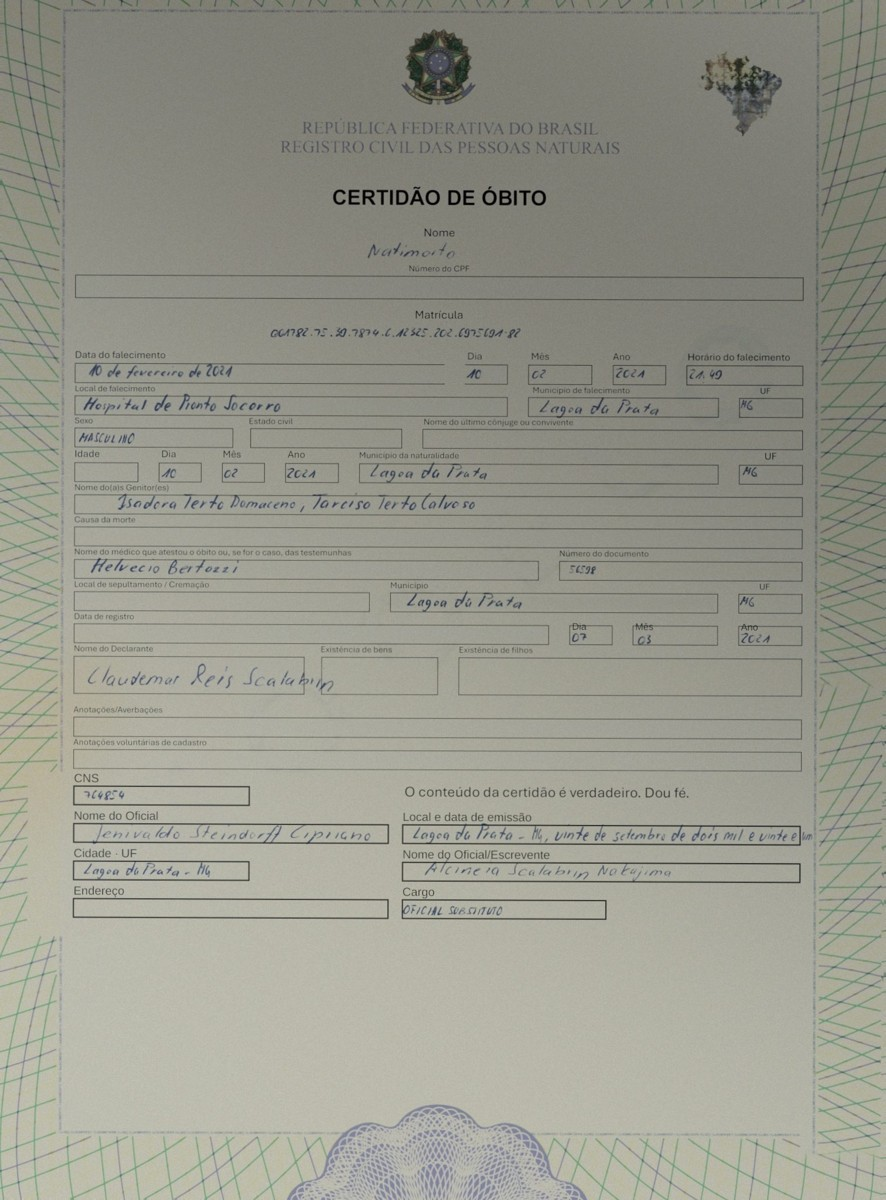
\includegraphics[height=0.76\textheight]{gerador_pagina.jpg}

\scriptsize Certidão de óbito do teste difícil, VATr++, nível 2
\end{column}
\begin{column}{0.64\textwidth}
\small
\begin{itemize}
  \item \textbf{Modelo}: modelos em branco e mapas de campos do OCRSD
  \item \textbf{Registro}: um registro do OCRSD re-sorteado; cada prenome, sobrenome e município troca na página inteira por um do léxico, respeitando a partição entre treino e teste
  \item \textbf{Mão}: uma mão e uma caneta por página, com 31 fontes manuscritas ou os geradores neurais VATr++ e Graves (estes só escrevem texto sem acento)
  \item \textbf{Dificuldade}: níveis 1 a 4, com letras deformadas e fundidas, falhas e borrões, papel com sombra, ruído e JPEG
\end{itemize}
\end{column}
\end{columns}
\end{frame}

\begin{frame}{Página gerada, em detalhe}
\centering
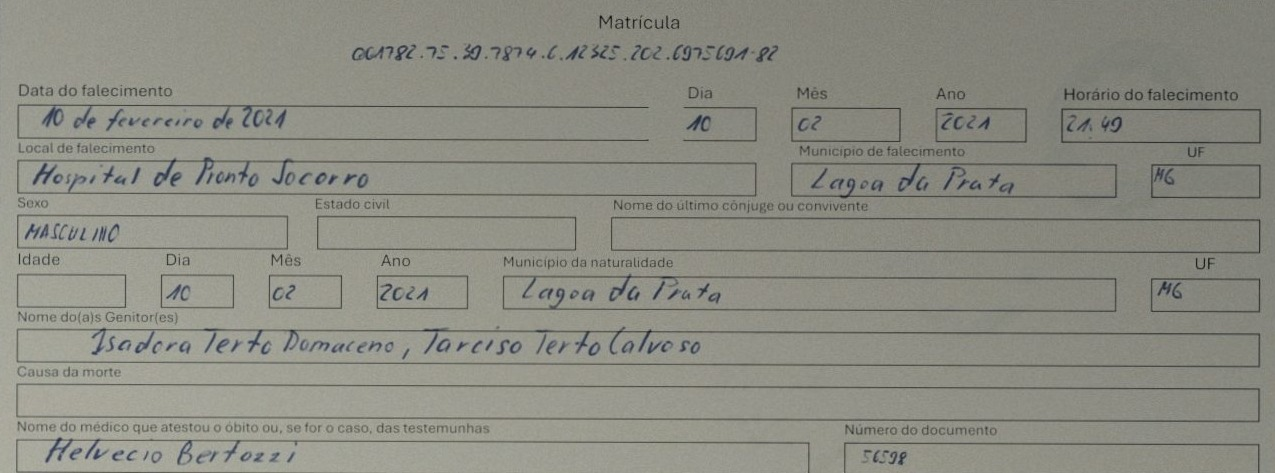
\includegraphics[width=0.80\textwidth]{gerador_zoom_1.jpg}

\vspace{0.4em}
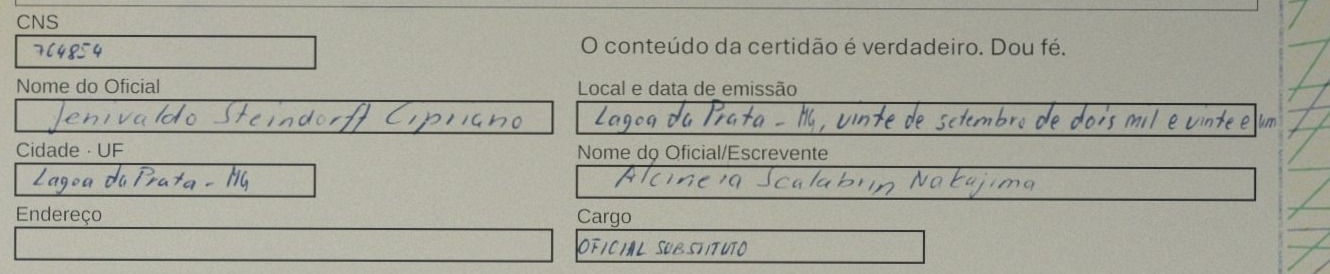
\includegraphics[width=0.80\textwidth]{gerador_zoom_2.jpg}
\end{frame}

\begin{frame}{Campos manuscritos certos: de 55\% para 72\%}
\centering
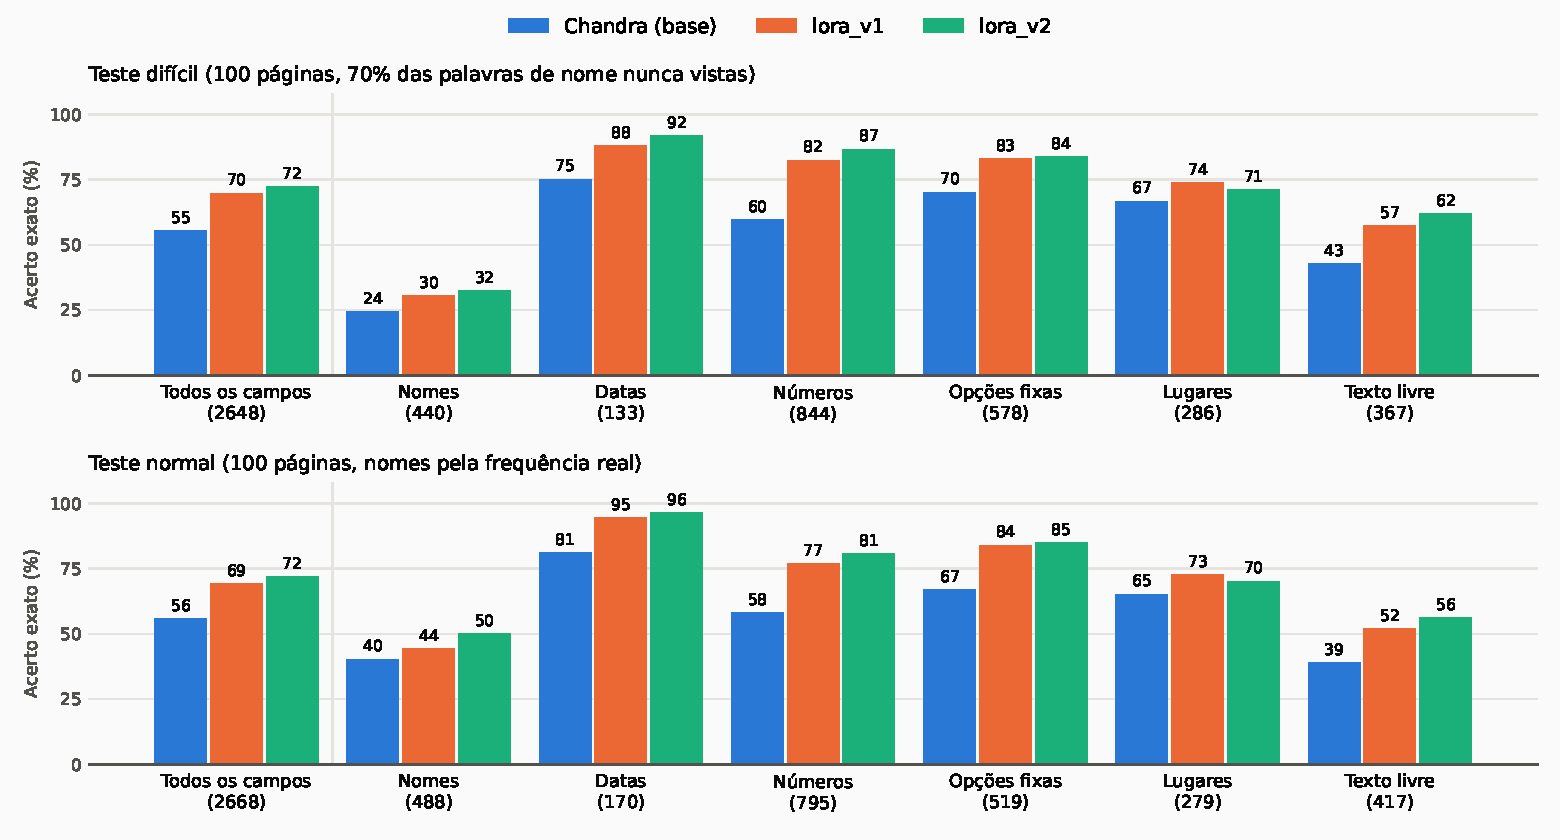
\includegraphics[width=0.82\textwidth]{resultados.pdf}

\vspace{-0.2em}
\scriptsize
lora\_v2 sobre o Chandra (difícil / normal): \textbf{+16,8 / +16,2} pontos nos campos, \textbf{+8,2 / +9,8} nos nomes; IC 95\% $>$ 0
\end{frame}

\begin{frame}{No gerador do ONR, com escritores fora do treino: de 85\% para 96\%}
\centering
\footnotesize
\begin{tabular}{@{}lrrr@{}}
\toprule
94 páginas do OCRSD, campos exatos (\%) & Campos & Chandra OCR 2 & lora\_v1 \\
\midrule
Todos os campos manuscritos & 1.460 & 84,6 & \textbf{95,5} \\
\quad Nomes & 399 & 84,7 & \textbf{95,5} \\
\quad Opções fixas (sexo, estado civil\dots) & 244 & 74,6 & \textbf{98,8} \\
\quad Texto livre & 286 & 72,7 & \textbf{91,3} \\
\quad Lugares & 132 & 93,2 & \textbf{98,5} \\
\quad Datas & 94 & 98,9 & 98,9 \\
\quad Números & 305 & \textbf{95,4} & 94,4 \\
\bottomrule
\end{tabular}

\vspace{0.4em}
\raggedright
\small
\begin{itemize}
  \item O lora\_v1 acertou 172 campos que o Chandra errava e errou 13 que ele acertava (IC 95\% da diferença: +8,1 a +14,0 pontos)
  \item Este teste mede caligrafia e layout de outro gerador; os nomes raros são medidos no teste local
\end{itemize}
\tiny Depois deste teste, essas páginas entraram no treino do lora\_v2, por isso ele não tem resultado aqui.
\end{frame}

\begin{frame}{Demonstração: o que o modelo devolve}
\begin{columns}[T]
\begin{column}{0.30\textwidth}
\centering
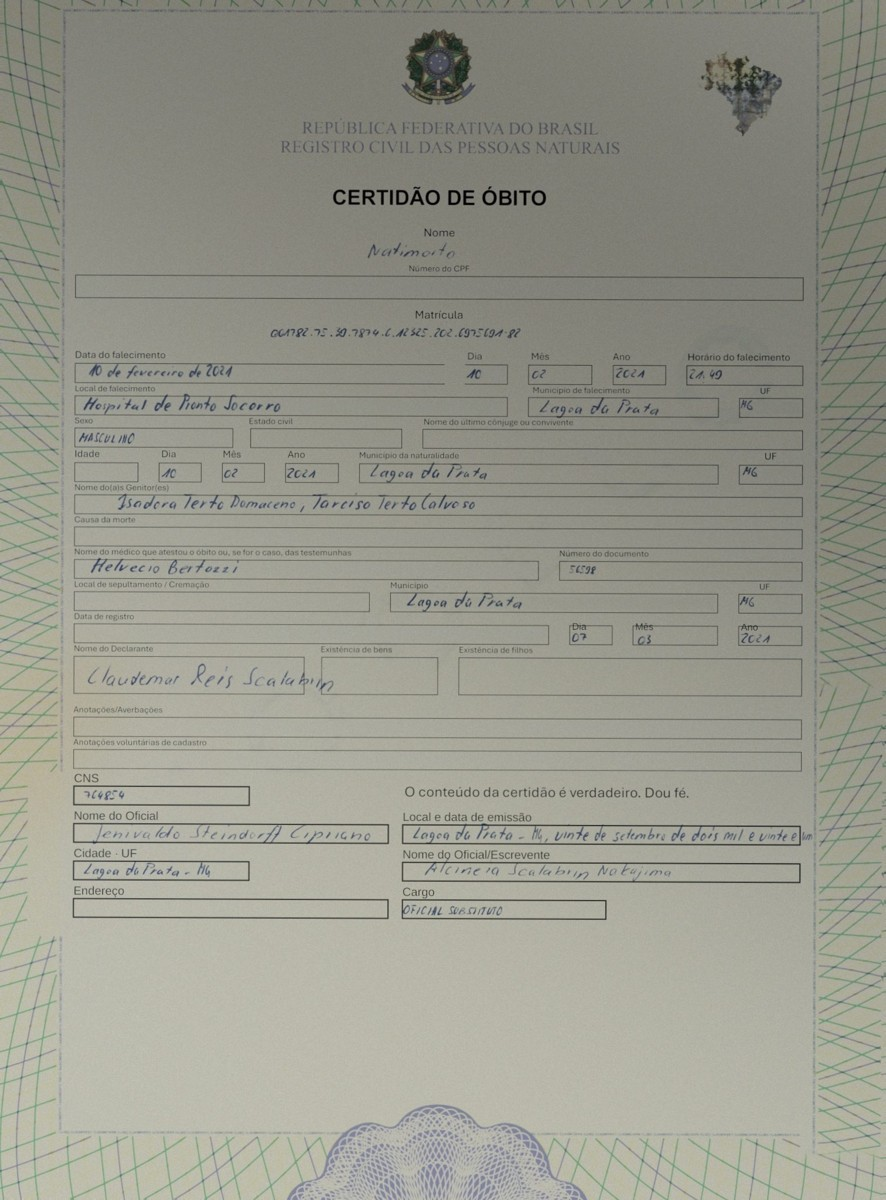
\includegraphics[height=0.78\textheight]{gerador_pagina.jpg}

\scriptsize Entrada
\end{column}
\begin{column}{0.30\textwidth}
\centering
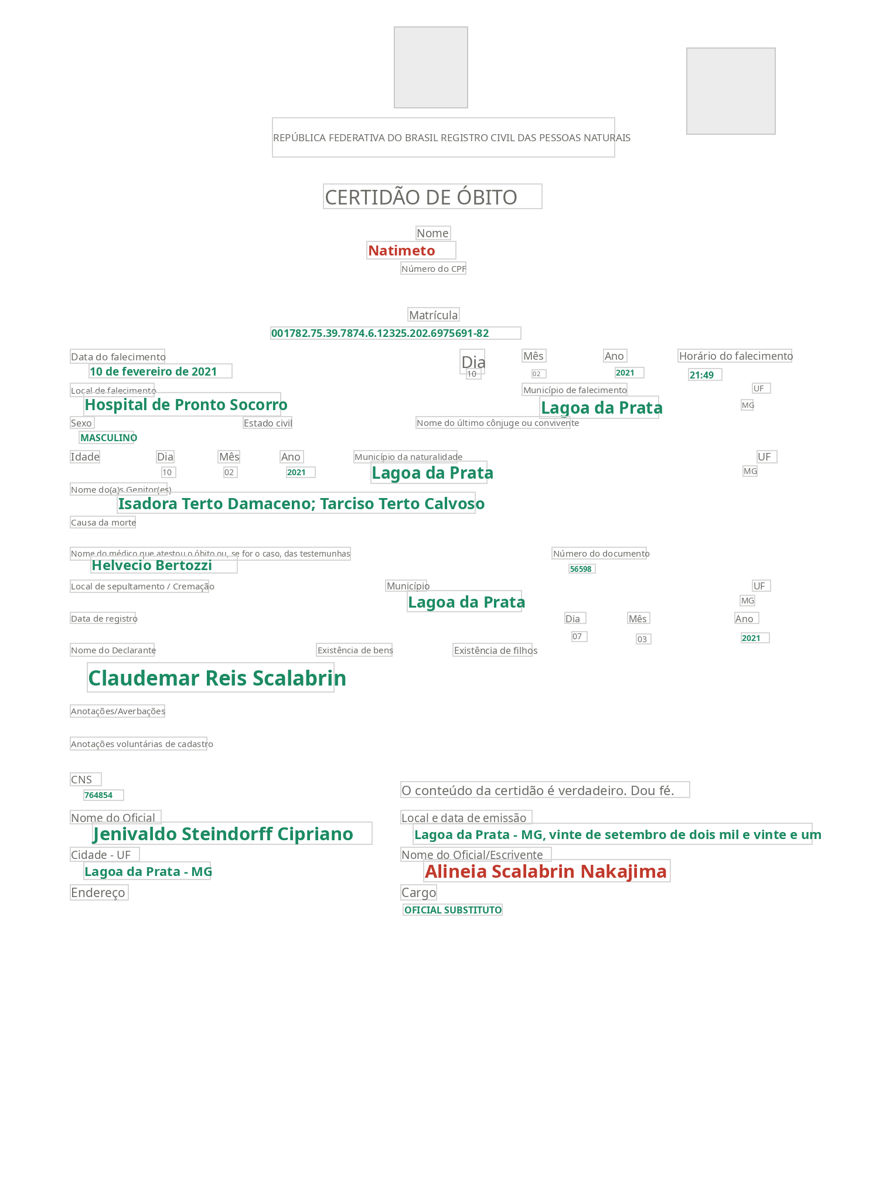
\includegraphics[height=0.78\textheight]{demo_lora_v2.png}

\scriptsize Saída do lora\_v2, redesenhada
\end{column}
\begin{column}{0.36\textwidth}
\small
Cada bloco da saída tem texto e posição na página.

\vspace{0.5em}
\ok{Verde}: campo manuscrito certo\\
\erro{Vermelho}: campo errado\\
Cinza: texto impresso
\vspace{0.6em}

\begin{tabular}{@{}lr@{}}
\toprule
Campos certos & de 22 \\
\midrule
Chandra OCR 2 & 17 \\
lora\_v2 & \textbf{20} \\
\bottomrule
\end{tabular}
\vspace{0.4em}

\scriptsize O Chandra errou a matrícula, o horário, dois nomes e um sobrenome; o lora\_v2 errou ``Natimorto'' e ``Alcineia''.
\end{column}
\end{columns}
\end{frame}

\begin{frame}{O erro que sobra: o prenome raro vira um prenome comum}
\footnotesize
\centering
\renewcommand{\arraystretch}{1.15}
\begin{tabular}{@{}m{4.0cm}m{3.3cm}m{3.4cm}m{2.0cm}@{}}
\toprule
Imagem & Gabarito & Chandra & lora\_v2 \\
\midrule
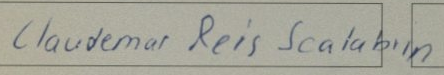
\includegraphics[width=3.8cm]{nome_1.png} & Claudemar Reis Scalabrin & Claude\erro{mi}r Reis Scalabrin & \ok{igual} \\
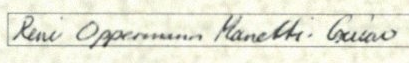
\includegraphics[width=3.8cm]{nome_2.png} & Reni Oppermann Manetti Guiao & \dots{} Manett\erro{e} \erro{Greco} & \ok{igual} \\
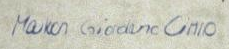
\includegraphics[width=2.8cm]{nome_3.png} & Maikon Giordano Cirino & \erro{Manoel} Giordan\erro{e} \erro{Critto} & \erro{Marcia} \dots \\

\includegraphics[width=3.6cm]{nome_4.png} & Guiomar Schiavon Arrabal & \erro{Geovana} Schiav\erro{e}n \dots & \erro{Giovana} \dots \\
\bottomrule
\end{tabular}

\vspace{0.5em}
\raggedright
No teste difícil, os nomes exatos subiram de 24,3\% para 32,5\%. O que ainda falha é o caso que motivou o projeto
\end{frame}

\begin{frame}{A versão quantizada mantém quase todo o ganho}
\scriptsize
\centering
\renewcommand{\arraystretch}{1.0}
\setlength{\tabcolsep}{5pt}
\begin{tabular}{@{}lcc|c|ccc@{}}
\toprule
 & \multicolumn{2}{c|}{\textbf{Chandra OCR 2}} & \textbf{lora\_v1} & \multicolumn{3}{c}{\textbf{lora\_v2}} \\
 & BF16 & FP8 & BF16 & BF16 & FP8 & INT4 \\
\midrule
\multicolumn{7}{@{}l}{\textit{Teste difícil (100 páginas)}} \\
\quad Campos exatos (\%) & 55,4 & 55,1 & 69,8 & \textbf{72,2} & 71,7 & 69,9 \\
\quad Nomes exatos (\%) & 24,3 & 24,3 & 30,5 & \textbf{32,5} & 30,7 & 28,9 \\
\multicolumn{7}{@{}l}{\textit{Teste normal (100 páginas)}} \\
\quad Campos exatos (\%) & 55,8 & -- & 69,2 & \textbf{72,0} & 71,9 & 71,6 \\
\quad Nomes exatos (\%) & 40,4 & -- & 44,5 & \textbf{50,2} & 49,6 & 49,4 \\
\multicolumn{7}{@{}l}{\textit{Inferência (RTX PRO 6000, vLLM)}} \\
\quad Pesos na GPU (GiB) $\downarrow$ & 8,6 & 6,2 & 8,6 & 8,6 & 6,2 & \textbf{5,0} \\
\quad Uma página por vez (s/página) $\downarrow$ & 23,0 & -- & -- & 22,6 & 17,7 & \textbf{14,9} \\
\quad 48 páginas por vez (s/página) $\downarrow$ & 1,25 & 1,20 & -- & 1,22 & 1,07 & \textbf{1,05} \\
\bottomrule
\end{tabular}

\vspace{0.3em}
\raggedright
\tiny
Negrito: melhor da linha. --: não medido. Uma página por vez: média de 3 páginas do teste difícil. O lora\_v1 leu o teste difícil numa L4; o resto rodou numa RTX PRO 6000.
\end{frame}

% ================================================================== fechamento
\begin{frame}{Segurança e privacidade}
\small
\begin{itemize}
  \item \textbf{Sem dados de pessoas reais no treino}: nomes entram só como contagens agregadas, e os registros das certidões são sintéticos (OCRSD e gerador local)
  \item \textbf{Sem sinal de memorização}: em linhas, o erro em nomes vistos e inéditos continuou com a mesma diferença (2,3 $\rightarrow$ 2,1 pontos)
  \item \textbf{Teste separado do treino}: nomes, fontes e escritores de teste ficam fora do treino; nenhuma página de teste foi usada para escolher parâmetros
  \item \textbf{Controle de saída}: saídas vazias, em laço ou com cara de instrução vão para revisão humana. Em linhas, as aprovadas tiveram CER de 1,0\%, contra 7,6\% nas enviadas para revisão
  \item \textbf{LGPD}: nenhuma certidão real foi usada; testar com documentos reais depende de autorização do controlador dos dados
\end{itemize}
\end{frame}

\begin{frame}{Desafios e limitações}
\begin{columns}[T]
\begin{column}{0.48\textwidth}
\small
\textbf{Desafios técnicos e como foram tratados}
\begin{itemize}
  \item O ganho em linhas não chegava à página: treino com páginas inteiras
  \item Os geradores neurais de escrita não escrevem acentos: usados só em texto sem acento; o texto acentuado vem das páginas com fontes
  \item O valor de um campo pode aparecer em qualquer lugar da saída: avaliação que localiza cada campo pela posição
\end{itemize}
\end{column}
\begin{column}{0.48\textwidth}
\small
\textbf{Limitações e próximo passo}
\begin{itemize}
  \item Nomes nunca vistos: 32,5\% exatos no teste difícil. Próximo passo: mais nomes raros no treino e revisão guiada pela confiança
  \item Fora das certidões, o Chandra original ainda lê melhor. Próximo passo: misturar outros tipos de página no treino
  \item Teste só com páginas sintéticas, nos 5 documentos do treino. Próximo passo: documentos reais, com autorização
\end{itemize}
\end{column}
\end{columns}
\end{frame}

\begin{frame}{Conclusão}
\begin{itemize}
  \item Treinar no formato em que o modelo é usado, a página inteira, foi o que levou o ganho para as certidões
  \item O Chandra ajustado passou de 55\% para 72\% dos campos manuscritos certos no nosso gerador e de 85\% para 96\% no OCRSD (lora\_v1), sem páginas truncadas ou em laço
  \item Em INT4, cabe em 5 GiB e lê uma certidão em cerca de 15 s
  \item \textbf{Contribuições}: léxico de nomes sem dados pessoais, gerador de certidões manuscritas, avaliador de campos em página inteira e os adaptadores treinados
\end{itemize}
\end{frame}

\begin{frame}[standout]
Obrigado!

\vspace{0.6em}
\normalsize
Agradecimentos ao tutor Lucas Mayr e ao ONR, pelo gerador OCRSD

\vspace{0.4em}
\texttt{github.com/gabriel-salmoria/ai-sec}
\end{frame}

% ================================================================== extras para perguntas
\appendix

\begin{frame}{Extra: documentos fora das certidões}
\small
\begin{tabular}{@{}lrrr@{}}
\toprule
& Chandra OCR 2 & lora\_v0 (linhas) & lora\_v2 (páginas) \\
\midrule
BRESSAY, 199 redações: CER (\%) $\downarrow$ & 26,5 & \textbf{17,3} & 48,6 \\
XFUND-PT, 50 formulários: campos (\%) & \textbf{53,0} & -- & 43,8 \\
\bottomrule
\end{tabular}

\vspace{0.6em}
\begin{itemize}
  \item No BRESSAY, 12 páginas do lora\_v2 e 13 do Chandra atingiram o limite de 6.144 \emph{tokens}; nas 181 em que nenhum dos dois atingiu, o CER foi de 6,8\% (Chandra) para 7,9\%
  \item No XFUND-PT, a ``letra manuscrita'' é desenhada com fontes, num layout que o treino não viu
  \item O lora\_v2 só viu certidões no treino; misturar outros documentos é o próximo passo
\end{itemize}
\end{frame}

\begin{frame}{Extra: detalhes do treino}
\small
\begin{tabular}{@{}lll@{}}
\toprule
& lora\_v1 & lora\_v2 \\
\midrule
Ponto de partida & Chandra OCR 2 & lora\_v1 \\
Páginas & 1.800 (941 locais, 859 OCRSD) & 1.700 (1.559 locais, 141 OCRSD) \\
Pesos na perda & impresso 0,3, manuscrito 1 & e nomes 2, com peso extra no erro \\
Tempo de treino & 66 min & 65 min \\
\bottomrule
\end{tabular}

\vspace{0.6em}
\begin{itemize}
  \item LoRA de posto 16 ($\alpha$ = 32) nas camadas lineares do modelo de linguagem; encoder de visão congelado
  \item Uma época, taxa de aprendizado $10^{-4}$, currículo das páginas mais limpas às mais degradadas
  \item Páginas com lado maior de 2.048 px; pico de 61 GB de memória na GPU
  \item Quantização sem dados de calibração: FP8 dinâmico e INT4 só nos pesos (W4A16), com o llm-compressor
\end{itemize}
\end{frame}

\end{document}
